\begin{example}{Sample-and-hold Feedback Control}
\label{ex:S&Hcontrol}
Consider a physical process modeled as in \IfSAE{Example 5.7}{Example~\ref{ex:LTIplant}}
and a state feedback interconnection.
The algorithm (static gain) uses measurements of its
output and controls the input of the physical process with the goal of steering its state to zero. 
Suppose the sampling device is ideal and that the signals are connected to the plant via a DAC modeled as 
\IfSAE
{
follows.
The digital signals in the cyber components need to be converted
to analog signals for their use in the physical world.
Digital-to-analog converters (DACs) perform such a task 
by converging digital signals into analog equivalents.
One of the most common models for a DAC
is the zero-order hold model (ZOH). In simple terms, a ZOH converts
a digital signal at its input into an analog signal 
at its output.  
Its output is updated at discrete time instants, typically periodically,
and held constant in between updates, until new information is available at the
next sampling time. We will model DACs as ZOH devices with similar dynamics. Let
$\tau_h\in\realsgeq$ be the timer state, $m_h \in \reals^{r_C}$ be the
sample state (note that the value of $h$ indicates the number of DACs
in the interface), and $v_h \in \reals^{r_C}$ be the inputs of the DAC.
Its operation is as follows. When $\tau_h \leq 0$, the timer state
is reset to $\tau_r$ and the sample state is updated with $v_h$ (usually
the output of the embedded computer), where $\tau_r\in[T^{\mbox{min}},T^{\mbox{max}}]$ is a random variable that models the time in-between communication instants and $T^{\mbox{min}}\leq T^{\mbox{max}}$.  A model that captures this
mechanism is given by 
\begin{eqnarray}\label{eqn:DACmodel-a}
\left.
\begin{array}{l}
\dot{\tau}_h =\ -1,   \ \
\dot{m}_h  =\ 0
\end{array}
\right. & \mbox{ when }& \tau_h \in [T^{\mbox{min}},T^{\mbox{max}}] \\ \label{eqn:DACmodel-b}
\left.
\begin{array}{ll}
\tau_h^+  =\ \tau_r,  \ \
m_h^+ =\ v_h
\end{array}
\right. & \mbox{ when }& \tau_h \leq T^{\mbox{min}}
\end{eqnarray}
}
{in \eqref{eqn:DACmodel-a}-\eqref{eqn:DACmodel-b}.}


The interconnection between the models of the physical process, the sampling device, the finite state 
machine, and the DAC has the feedback topology shown in Figure~\ref{fig:S&Hcontrol}.  In particular, the output of the DAC is connected to the input $\up$ of the physical process by a matrix gain $K$, while the input $\uc$ of the finite state machine is equal to the output $\yp$ of the physical process
at every sampling instant. 
\begin{itemize}
\item Physical process:
\begin{eqnarray}
\fp(\xp, u):= A\xp + Bu,\ 
   \Cp : = \Re^{2}\times\Re^{2},\\
\gp(\xp, u):= \xp,\ 
    \Dp: =\emptyset,\ 
\yp = h(\xp) : =x
\end{eqnarray}
where $A = \begin{bmatrix}0 & 1 \\ 0 & -b/m\end{bmatrix}$, $B = \begin{bmatrix}1 & 1/m\end{bmatrix}$, and $x=(x_1,x_2)\in\Re^{2}$.

\item Analog-to-Digital Converter (ADC):
\begin{eqnarray}
f(x, u):= \begin{bmatrix}0\\0\\1\end{bmatrix},\ 
   C : = \defset{(x,u)}{ \tau_s \in [0,T^*_s] },\\
g(x, u):= \begin{bmatrix} u\\ 0\end{bmatrix},\ 
    D: =\defset{(x,u)}{ \tau_s \geq T^*_s },\ 
y = h(x) : =x
\end{eqnarray}
where $x=(m_s,\tau_s)\in\Re\times\Re^{2}$, and $u\in\Re^{2}$.

\item Zero-Order Hold (ZOH):
\begin{eqnarray}
f(x, u):= \begin{bmatrix}0\\0\\1\end{bmatrix},\ 
   C : = \defset{(x,u)}{ \tau_s \in [0,T^*_s] },\\
g(x, u):= \begin{bmatrix} u\\ 0\end{bmatrix},\ 
    D: =\defset{(x,u)}{ \tau_s \geq T^*_s },\ 
y = h(x) : =x
\end{eqnarray}
where $x=(m_s,\tau_s)\in\Re\times\Re^{2}$, and $u\in\Re^{2}$.

\end{itemize}

The feedback gain is given by $K = \begin{bmatrix}k_1\\k_2\end{bmatrix}$. 
%\begin{eqnarray}
%f(x, u):= ,\ 
%   C : = \defset{(x,u)}{ },\\
%g(x, u):= ,\ 
%    D: =\defset{(x,u)}{ },\ 
%y = h(x) : =x
%\end{eqnarray}


\begin{figure}[ht!]
  \begin{center}
    {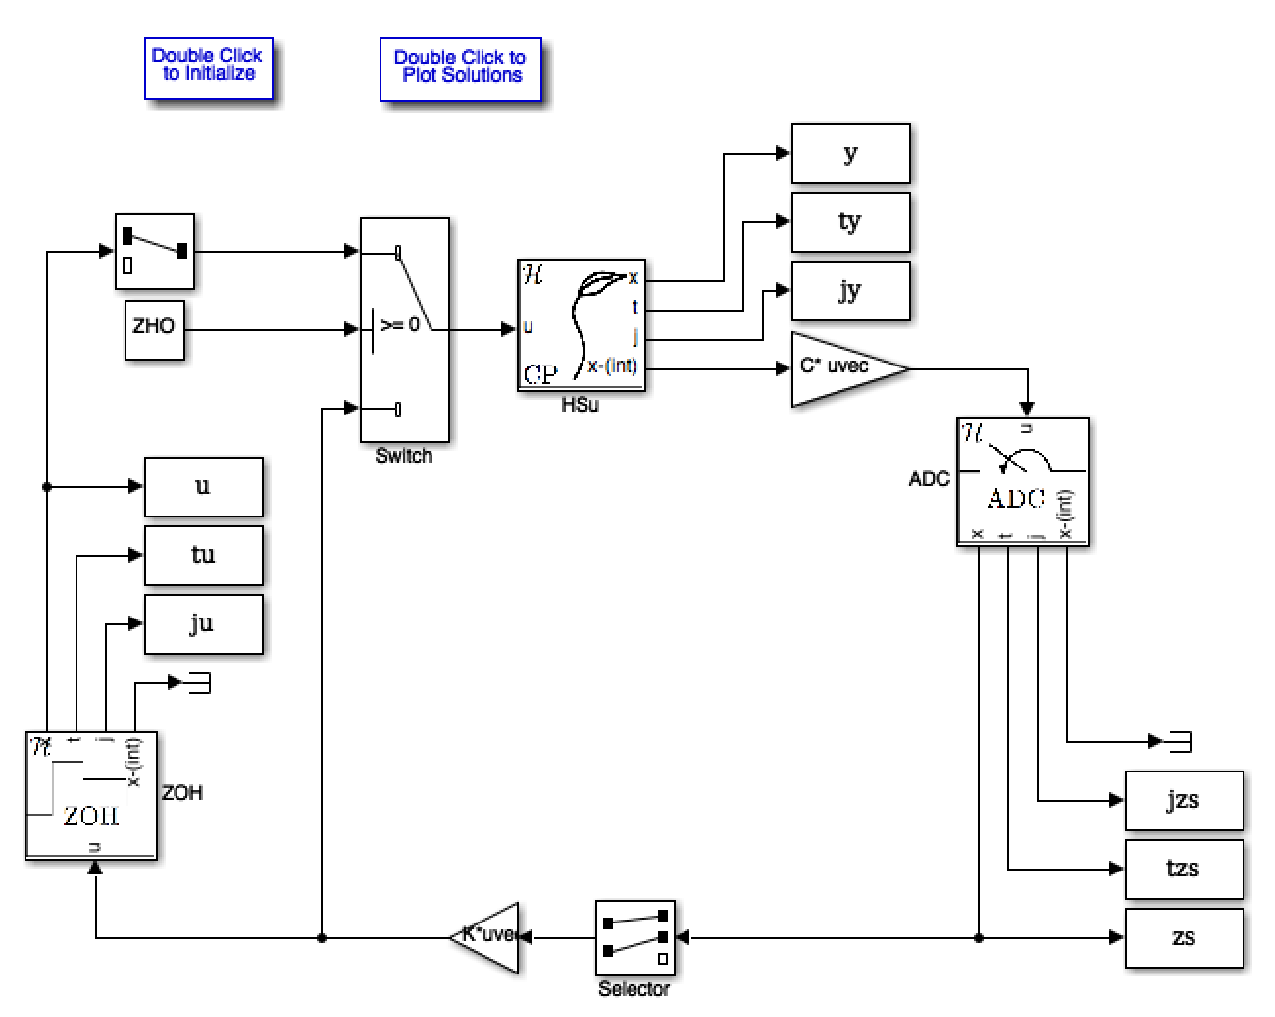
\includegraphics[width=0.8\textwidth]{figures/Simulink/SampleandHoldExample.eps}}
   \caption{Sample and hold feedback interconnection for Example~\ref{ex:S&Hcontrol}}
\label{fig:S&Hcontrol}
  \end{center}
\end{figure}

For each hybrid system in Figure~\ref{fig:S&Hcontrol} (HSu, ADC, and ZOH) we have the following Matlab embedded functions that describe the sets $C$ and $D$ and functions $f$ and $g$.
Figure~\ref{fig:ZOH_exampleResults} presents a numerical simulation of the interconnected system.

\begin{figure}%[ht]
  \begin{center}
    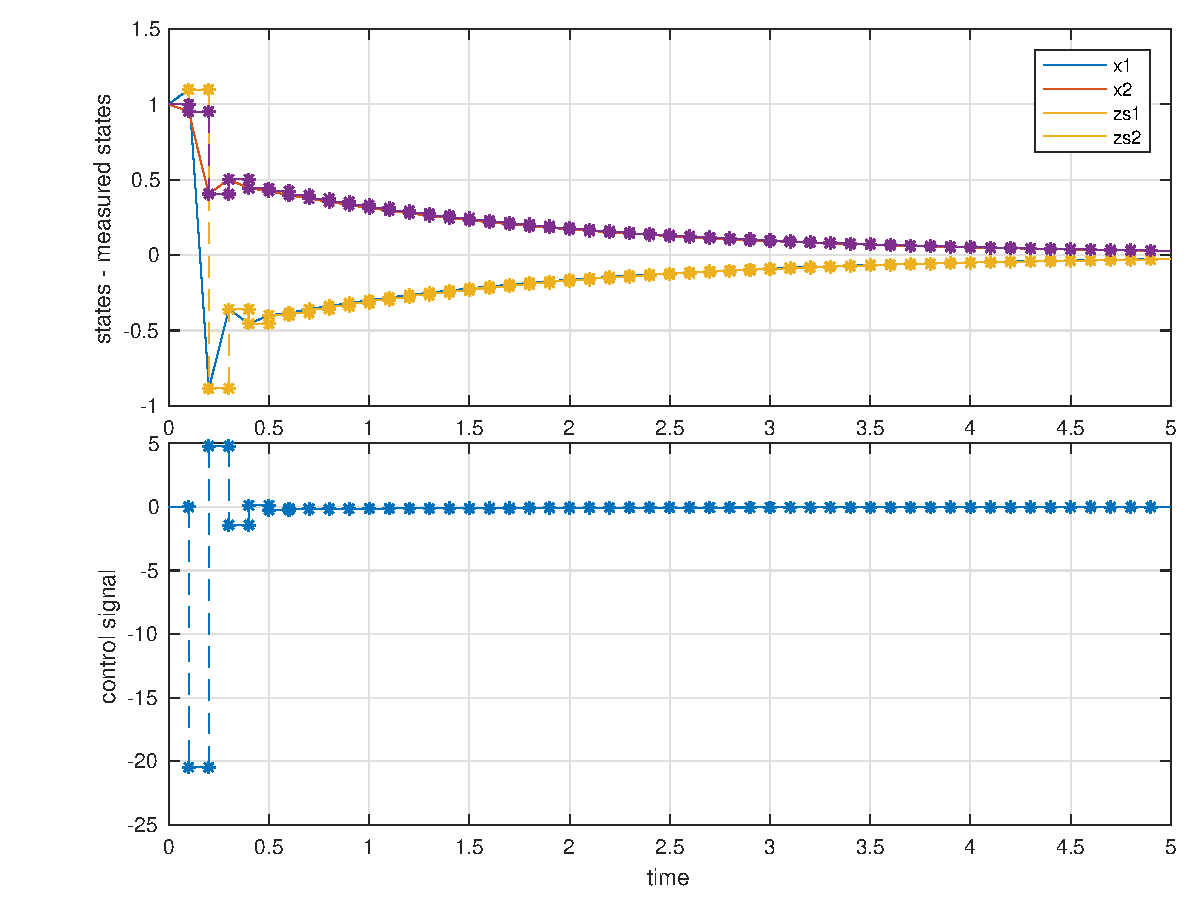
\includegraphics[width=0.8\textwidth]{figures/Simulink/ZOH_exampleResults.eps}
   \caption{Measuread states and inputs.}
\label{fig:ZOH_exampleResults}
  \end{center}
\end{figure}

% Set the location for MATLAB files included via the "\code" command.
\codeLocation{Matlab2tex_CPS_ContinuousPlant}

\begin{itemize}
\item Continuous process:

\code{f.m}
\code{C.m}
\code{g.m}
\code{D.m}

% Flow map
% %\scriptsize
% % This file was automatically created from the m-file 
% "m2tex.m" written by USL. 
% The fontencoding in this file is UTF-8. 
%  
% You will need to include the following two packages in 
% your LaTeX-Main-File. 
%  
% \usepackage{color} 
% \usepackage{fancyvrb} 
%  
% It is advised to use the following option for Inputenc 
% \usepackage[utf8]{inputenc} 
%  
  
% definition of matlab colors: 
\definecolor{mblue}{rgb}{0,0,1} 
\definecolor{mgreen}{rgb}{0.13333,0.5451,0.13333} 
\definecolor{mred}{rgb}{0.62745,0.12549,0.94118} 
\definecolor{mgrey}{rgb}{0.5,0.5,0.5} 
\definecolor{mdarkgrey}{rgb}{0.25,0.25,0.25} 
  
\DefineShortVerb[fontfamily=courier,fontseries=m]{\$} 
\DefineShortVerb[fontfamily=courier,fontseries=b]{\#} 
  
\noindent                    
 \hspace*{-1.6em}{\scriptsize 1}$  $\color{mblue}$function$\color{black}$ xdot = f(x, u, gamma)$\\
 \hspace*{-1.6em}{\scriptsize 2}$  $\\
 \hspace*{-1.6em}{\scriptsize 3}$  $\color{mgreen}#%%%%%%%%%%%%%%%%%%%%%%%%%%%%%%%%%%%%%%%%%%%%%%%%%%%%%%%%%%%%%%%%%%%%%%%%%%%#\color{black}$$\\
 \hspace*{-1.6em}{\scriptsize 4}$  $\color{mgreen}$% Matlab Function  Author: Ricardo Sanfelice $\color{black}$$\\
 \hspace*{-1.6em}{\scriptsize 5}$  $\color{mgreen}$% (Revised by Giampiero Campa)$\color{black}$$\\
 \hspace*{-1.6em}{\scriptsize 6}$  $\color{mgreen}$% (Revised by Pablo Nanez)$\color{black}$$\\
 \hspace*{-1.6em}{\scriptsize 7}$  $\color{mgreen}$%$\color{black}$$\\
 \hspace*{-1.6em}{\scriptsize 8}$  $\color{mgreen}$% Project: Simulation of a hybrid system (Bouncing Ball)$\color{black}$$\\
 \hspace*{-1.6em}{\scriptsize 9}$  $\color{mgreen}$%$\color{black}$$\\
 \hspace*{-2em}{\scriptsize 10}$  $\color{mgreen}$% Name: f.m$\color{black}$$\\
 \hspace*{-2em}{\scriptsize 11}$  $\color{mgreen}$%$\color{black}$$\\
 \hspace*{-2em}{\scriptsize 12}$  $\color{mgreen}$% Description: Flow map$\color{black}$$\\
 \hspace*{-2em}{\scriptsize 13}$  $\color{mgreen}$%$\color{black}$$\\
 \hspace*{-2em}{\scriptsize 14}$  $\color{mgreen}$% Version: 1.0$\color{black}$$\\
 \hspace*{-2em}{\scriptsize 15}$  $\color{mgreen}$% Required files: - $\color{black}$$\\
 \hspace*{-2em}{\scriptsize 16}$  $\color{mgreen}#%%%%%%%%%%%%%%%%%%%%%%%%%%%%%%%%%%%%%%%%%%%%%%%%%%%%%%%%%%%%%%%%%%%%%%%%%%%#\color{black}$$\\
 \hspace*{-2em}{\scriptsize 17}$  $\\
 \hspace*{-2em}{\scriptsize 18}$  $\\
 \hspace*{-2em}{\scriptsize 19}$  $\color{mgreen}$% flow map: xdot=f(x,u);$\color{black}$$\\
 \hspace*{-2em}{\scriptsize 20}$  xdot = [x(2); gamma];$\\ 
  
\UndefineShortVerb{\$} 
\UndefineShortVerb{\#}\label{scr:f}
% %\normalsize

% Flow set
% %\scriptsize
% % This file was automatically created from the m-file 
% "m2tex.m" written by USL. 
% The fontencoding in this file is UTF-8. 
%  
% You will need to include the following two packages in 
% your LaTeX-Main-File. 
%  
% \usepackage{color} 
% \usepackage{fancyvrb} 
%  
% It is advised to use the following option for Inputenc 
% \usepackage[utf8]{inputenc} 
%  
  
% definition of matlab colors: 
\definecolor{mblue}{rgb}{0,0,1} 
\definecolor{mgreen}{rgb}{0.13333,0.5451,0.13333} 
\definecolor{mred}{rgb}{0.62745,0.12549,0.94118} 
\definecolor{mgrey}{rgb}{0.5,0.5,0.5} 
\definecolor{mdarkgrey}{rgb}{0.25,0.25,0.25} 
  
\DefineShortVerb[fontfamily=courier,fontseries=m]{\$} 
\DefineShortVerb[fontfamily=courier,fontseries=b]{\#} 
  
\noindent                          
 \hspace*{-1.6em}{\scriptsize 1}$  $\color{mblue}$function$\color{black}$ v  = C(x, u)$\\
 \hspace*{-1.6em}{\scriptsize 2}$  $\color{mgreen}$%--------------------------------------------------------------------------$\color{black}$$\\
 \hspace*{-1.6em}{\scriptsize 3}$  $\color{mgreen}$% Matlab M-file Project: HyEQ Toolbox @  Hybrid Systems Laboratory (HSL),$\color{black}$$\\
 \hspace*{-1.6em}{\scriptsize 4}$  $\color{mgreen}$% https://hybrid.soe.ucsc.edu/software$\color{black}$$\\
 \hspace*{-1.6em}{\scriptsize 5}$  $\color{mgreen}$% http://hybridsimulator.wordpress.com/$\color{black}$$\\
 \hspace*{-1.6em}{\scriptsize 6}$  $\color{mgreen}$%--------------------------------------------------------------------------$\color{black}$$\\
 \hspace*{-1.6em}{\scriptsize 7}$  $\color{mgreen}$% Project: Simulation of a hybrid system$\color{black}$$\\
 \hspace*{-1.6em}{\scriptsize 8}$  $\color{mgreen}$% Description: Flow set$\color{black}$$\\
 \hspace*{-1.6em}{\scriptsize 9}$  $\color{mgreen}$%--------------------------------------------------------------------------$\color{black}$$\\
 \hspace*{-2em}{\scriptsize 10}$  $\color{mgreen}$%--------------------------------------------------------------------------$\color{black}$$\\
 \hspace*{-2em}{\scriptsize 11}$  $\color{mgreen}$%   See also HYEQSOLVER, PLOTARC, PLOTARC3, PLOTFLOWS, PLOTHARC,$\color{black}$$\\
 \hspace*{-2em}{\scriptsize 12}$  $\color{mgreen}$%   PLOTHARCCOLOR, PLOTHARCCOLOR3D, PLOTHYBRIDARC, PLOTJUMPS.$\color{black}$$\\
 \hspace*{-2em}{\scriptsize 13}$  $\color{mgreen}$%   Copyright @ Hybrid Systems Laboratory (HSL),$\color{black}$$\\
 \hspace*{-2em}{\scriptsize 14}$  $\color{mgreen}$%   Revision: 0.0.0.3 Date: 05/20/2015 3:42:00$\color{black}$$\\
 \hspace*{-2em}{\scriptsize 15}$  $\color{mgreen}$%$\color{black}$$\\
 \hspace*{-2em}{\scriptsize 16}$  $\color{mgreen}$% Check on flow conditions$\color{black}$$\\
 \hspace*{-2em}{\scriptsize 17}$  $\color{mgreen}$% E.g.,$\color{black}$$\\
 \hspace*{-2em}{\scriptsize 18}$  $\color{mgreen}$% if (x(1) >= u(1))  % flow condition$\color{black}$$\\
 \hspace*{-2em}{\scriptsize 19}$  $\color{mgreen}$%     v = 1;  % report flow$\color{black}$$\\
 \hspace*{-2em}{\scriptsize 20}$  $\color{mgreen}$% else$\color{black}$$\\
 \hspace*{-2em}{\scriptsize 21}$  $\color{mgreen}$%     v = 0;   % do not report flow$\color{black}$$\\
 \hspace*{-2em}{\scriptsize 22}$  $\color{mgreen}$% end$\color{black}$$\\
 \hspace*{-2em}{\scriptsize 23}$  $\\
 \hspace*{-2em}{\scriptsize 24}$  $\\
 \hspace*{-2em}{\scriptsize 25}$  v = 1; $\color{mgreen}$% report flow$\color{black}$$\\
 \hspace*{-2em}{\scriptsize 26}$  $\\ 
  
\UndefineShortVerb{\$} 
\UndefineShortVerb{\#}\label{scr:C}
% %\normalsize

% Jump map
% %\scriptsize
% % This file was automatically created from the m-file 
% "m2tex.m" written by USL. 
% The fontencoding in this file is UTF-8. 
%  
% You will need to include the following two packages in 
% your LaTeX-Main-File. 
%  
% \usepackage{color} 
% \usepackage{fancyvrb} 
%  
% It is advised to use the following option for Inputenc 
% \usepackage[utf8]{inputenc} 
%  
  
% definition of matlab colors: 
\definecolor{mblue}{rgb}{0,0,1} 
\definecolor{mgreen}{rgb}{0.13333,0.5451,0.13333} 
\definecolor{mred}{rgb}{0.62745,0.12549,0.94118} 
\definecolor{mgrey}{rgb}{0.5,0.5,0.5} 
\definecolor{mdarkgrey}{rgb}{0.25,0.25,0.25} 
  
\DefineShortVerb[fontfamily=courier,fontseries=m]{\$} 
\DefineShortVerb[fontfamily=courier,fontseries=b]{\#} 
  
\noindent   
 \hspace*{-1.6em}{\scriptsize 1}$  $\color{mblue}$function$\color{black}$ xplus = g(x, u, lambda)$\\
 \hspace*{-1.6em}{\scriptsize 2}$  $\color{mgreen}$% jump map$\color{black}$$\\
 \hspace*{-1.6em}{\scriptsize 3}$  xplus = [u(1); -lambda*x(2)];$\\ 
  
\UndefineShortVerb{\$} 
\UndefineShortVerb{\#}\label{scr:g}
% %\normalsize

% Jump set
% %\scriptsize
% % This file was automatically created from the m-file 
% "m2tex.m" written by USL. 
% The fontencoding in this file is UTF-8. 
%  
% You will need to include the following two packages in 
% your LaTeX-Main-File. 
%  
% \usepackage{color} 
% \usepackage{fancyvrb} 
%  
% It is advised to use the following option for Inputenc 
% \usepackage[utf8]{inputenc} 
%  
  
% definition of matlab colors: 
\definecolor{mblue}{rgb}{0,0,1} 
\definecolor{mgreen}{rgb}{0.13333,0.5451,0.13333} 
\definecolor{mred}{rgb}{0.62745,0.12549,0.94118} 
\definecolor{mgrey}{rgb}{0.5,0.5,0.5} 
\definecolor{mdarkgrey}{rgb}{0.25,0.25,0.25} 
  
\DefineShortVerb[fontfamily=courier,fontseries=m]{\$} 
\DefineShortVerb[fontfamily=courier,fontseries=b]{\#} 
  
\noindent                         
 \hspace*{-1.6em}{\scriptsize 1}$  $\color{mblue}$function$\color{black}$ v  = D(x, u) $\\
 \hspace*{-1.6em}{\scriptsize 2}$  $\\
 \hspace*{-1.6em}{\scriptsize 3}$  $\color{mgreen}#%%%%%%%%%%%%%%%%%%%%%%%%%%%%%%%%%%%%%%%%%%%%%%%%%%%%%%%%%%%%%%%%%%%%%%%%%%%#\color{black}$$\\
 \hspace*{-1.6em}{\scriptsize 4}$  $\color{mgreen}$% Matlab Function  Author: Ricardo Sanfelice $\color{black}$$\\
 \hspace*{-1.6em}{\scriptsize 5}$  $\color{mgreen}$% (Revised by Giampiero Campa)$\color{black}$$\\
 \hspace*{-1.6em}{\scriptsize 6}$  $\color{mgreen}$% (Revised by Pablo Nanez)$\color{black}$$\\
 \hspace*{-1.6em}{\scriptsize 7}$  $\color{mgreen}$%$\color{black}$$\\
 \hspace*{-1.6em}{\scriptsize 8}$  $\color{mgreen}$% Project: Simulation of a hybrid system (Bouncing ball)$\color{black}$$\\
 \hspace*{-1.6em}{\scriptsize 9}$  $\color{mgreen}$%$\color{black}$$\\
 \hspace*{-2em}{\scriptsize 10}$  $\color{mgreen}$% Name: D.m$\color{black}$$\\
 \hspace*{-2em}{\scriptsize 11}$  $\color{mgreen}$%$\color{black}$$\\
 \hspace*{-2em}{\scriptsize 12}$  $\color{mgreen}$% Description: Jump set$\color{black}$$\\
 \hspace*{-2em}{\scriptsize 13}$  $\color{mgreen}$%$\color{black}$$\\
 \hspace*{-2em}{\scriptsize 14}$  $\color{mgreen}$% Version: 1.0$\color{black}$$\\
 \hspace*{-2em}{\scriptsize 15}$  $\color{mgreen}$% Required files: - $\color{black}$$\\
 \hspace*{-2em}{\scriptsize 16}$  $\color{mgreen}#%%%%%%%%%%%%%%%%%%%%%%%%%%%%%%%%%%%%%%%%%%%%%%%%%%%%%%%%%%%%%%%%%%%%%%%%%%%#\color{black}$$\\
 \hspace*{-2em}{\scriptsize 17}$  $\\
 \hspace*{-2em}{\scriptsize 18}$  xtemp = zeros(2,1);$\\
 \hspace*{-2em}{\scriptsize 19}$  xtemp = x;$\\
 \hspace*{-2em}{\scriptsize 20}$  $\\
 \hspace*{-2em}{\scriptsize 21}$  $\color{mblue}$if$\color{black}$ (xtemp(1) <= u(1)) && (xtemp(2) <= 0)  $\color{mgreen}$% jump condition$\color{black}$$\\
 \hspace*{-2em}{\scriptsize 22}$      v = 1;  $\color{mgreen}$% report jump$\color{black}$$\\
 \hspace*{-2em}{\scriptsize 23}$  $\color{mblue}$else$\color{black}$$\\
 \hspace*{-2em}{\scriptsize 24}$      v = 0;   $\color{mgreen}$% do not report jump$\color{black}$$\\
 \hspace*{-2em}{\scriptsize 25}$  $\color{mblue}$end$\color{black}$$\\ 
  
\UndefineShortVerb{\$} 
\UndefineShortVerb{\#}\label{scr:D}
% %\normalsize
\item ADC and ZOH:

\code{f\_ADC.m}
\code{C\_ADC.m}
\code{g\_ADC.m}
\code{D\_ADC.m}

% Flow map
% %\scriptsize
% % This file was automatically created from the m-file 
% "m2tex.m" written by USL. 
% The fontencoding in this file is UTF-8. 
%  
% You will need to include the following two packages in 
% your LaTeX-Main-File. 
%  
% \usepackage{color} 
% \usepackage{fancyvrb} 
%  
% It is advised to use the following option for Inputenc 
% \usepackage[utf8]{inputenc} 
%  
  
% definition of matlab colors: 
\definecolor{mblue}{rgb}{0,0,1} 
\definecolor{mgreen}{rgb}{0.13333,0.5451,0.13333} 
\definecolor{mred}{rgb}{0.62745,0.12549,0.94118} 
\definecolor{mgrey}{rgb}{0.5,0.5,0.5} 
\definecolor{mdarkgrey}{rgb}{0.25,0.25,0.25} 
  
\DefineShortVerb[fontfamily=courier,fontseries=m]{\$} 
\DefineShortVerb[fontfamily=courier,fontseries=b]{\#} 
  
\noindent                     
 \hspace*{-1.6em}{\scriptsize 1}$  $\color{mblue}$function$\color{black}$ xdot = f(x,vs)$\\
 \hspace*{-1.6em}{\scriptsize 2}$  $\color{mgreen}$%--------------------------------------------------------------------------$\color{black}$$\\
 \hspace*{-1.6em}{\scriptsize 3}$  $\color{mgreen}$% Matlab M-file Project: HyEQ Toolbox @  Hybrid Systems Laboratory (HSL), $\color{black}$$\\
 \hspace*{-1.6em}{\scriptsize 4}$  $\color{mgreen}$% https://hybrid.soe.ucsc.edu/software$\color{black}$$\\
 \hspace*{-1.6em}{\scriptsize 5}$  $\color{mgreen}$% http://hybridsimulator.wordpress.com/$\color{black}$$\\
 \hspace*{-1.6em}{\scriptsize 6}$  $\color{mgreen}$%--------------------------------------------------------------------------$\color{black}$$\\
 \hspace*{-1.6em}{\scriptsize 7}$  $\color{mgreen}$% Project: Simulation of a hybrid system Analog-to-Digital converter (ADC) $\color{black}$$\\
 \hspace*{-1.6em}{\scriptsize 8}$  $\color{mgreen}$% Description: Flow map$\color{black}$$\\
 \hspace*{-1.6em}{\scriptsize 9}$  $\color{mgreen}$%--------------------------------------------------------------------------$\color{black}$$\\
 \hspace*{-2em}{\scriptsize 10}$  $\color{mgreen}$%--------------------------------------------------------------------------$\color{black}$$\\
 \hspace*{-2em}{\scriptsize 11}$  $\color{mgreen}$%   See also HYEQSOLVER, PLOTARC, PLOTARC3, PLOTFLOWS, PLOTHARC,$\color{black}$$\\
 \hspace*{-2em}{\scriptsize 12}$  $\color{mgreen}$%   PLOTHARCCOLOR, PLOTHARCCOLOR3D, PLOTHYBRIDARC, PLOTJUMPS.$\color{black}$$\\
 \hspace*{-2em}{\scriptsize 13}$  $\color{mgreen}$%   Copyright @ Hybrid Systems Laboratory (HSL),$\color{black}$$\\
 \hspace*{-2em}{\scriptsize 14}$  $\color{mgreen}$%   Revision: 0.0.0.3 Date: 05/20/2015 3:42:00$\color{black}$$\\
 \hspace*{-2em}{\scriptsize 15}$  $\\
 \hspace*{-2em}{\scriptsize 16}$  n = length(vs); $\color{mgreen}$% measured input size$\color{black}$$\\
 \hspace*{-2em}{\scriptsize 17}$  $\\
 \hspace*{-2em}{\scriptsize 18}$  msdot = zeros(n,1); $\color{mgreen}$% measured continuous dynamics$\color{black}$$\\
 \hspace*{-2em}{\scriptsize 19}$  tau_sdot = 1; $\color{mgreen}$% Timer tau_s$\color{black}$$\\
 \hspace*{-2em}{\scriptsize 20}$  xdot = [msdot;tau_sdot];$\\
 \hspace*{-2em}{\scriptsize 21}$  $\\ 
  
\UndefineShortVerb{\$} 
\UndefineShortVerb{\#}\label{scr:f}
% %\normalsize

% Flow set
% %\scriptsize
% % This file was automatically created from the m-file 
% "m2tex.m" written by USL. 
% The fontencoding in this file is UTF-8. 
%  
% You will need to include the following two packages in 
% your LaTeX-Main-File. 
%  
% \usepackage{color} 
% \usepackage{fancyvrb} 
%  
% It is advised to use the following option for Inputenc 
% \usepackage[utf8]{inputenc} 
%  
  
% definition of matlab colors: 
\definecolor{mblue}{rgb}{0,0,1} 
\definecolor{mgreen}{rgb}{0.13333,0.5451,0.13333} 
\definecolor{mred}{rgb}{0.62745,0.12549,0.94118} 
\definecolor{mgrey}{rgb}{0.5,0.5,0.5} 
\definecolor{mdarkgrey}{rgb}{0.25,0.25,0.25} 
  
\DefineShortVerb[fontfamily=courier,fontseries=m]{\$} 
\DefineShortVerb[fontfamily=courier,fontseries=b]{\#} 
  
\noindent                                  
 \hspace*{-1.6em}{\scriptsize 1}$  $\color{mblue}$function$\color{black}$ v  = C(x, vs, Ts) $\\
 \hspace*{-1.6em}{\scriptsize 2}$  $\color{mgreen}$%--------------------------------------------------------------------------$\color{black}$$\\
 \hspace*{-1.6em}{\scriptsize 3}$  $\color{mgreen}$% Matlab M-file Project: HyEQ Toolbox @  Hybrid Systems Laboratory (HSL), $\color{black}$$\\
 \hspace*{-1.6em}{\scriptsize 4}$  $\color{mgreen}$% https://hybrid.soe.ucsc.edu/software$\color{black}$$\\
 \hspace*{-1.6em}{\scriptsize 5}$  $\color{mgreen}$% http://hybridsimulator.wordpress.com/$\color{black}$$\\
 \hspace*{-1.6em}{\scriptsize 6}$  $\color{mgreen}$%--------------------------------------------------------------------------$\color{black}$$\\
 \hspace*{-1.6em}{\scriptsize 7}$  $\color{mgreen}$% Project: Simulation of a hybrid system Analog-to-Digital converter (ADC) $\color{black}$$\\
 \hspace*{-1.6em}{\scriptsize 8}$  $\color{mgreen}$% Description: Flow set$\color{black}$$\\
 \hspace*{-1.6em}{\scriptsize 9}$  $\color{mgreen}$%--------------------------------------------------------------------------$\color{black}$$\\
 \hspace*{-2em}{\scriptsize 10}$  $\color{mgreen}$%--------------------------------------------------------------------------$\color{black}$$\\
 \hspace*{-2em}{\scriptsize 11}$  $\color{mgreen}$%   See also HYEQSOLVER, PLOTARC, PLOTARC3, PLOTFLOWS, PLOTHARC,$\color{black}$$\\
 \hspace*{-2em}{\scriptsize 12}$  $\color{mgreen}$%   PLOTHARCCOLOR, PLOTHARCCOLOR3D, PLOTHYBRIDARC, PLOTJUMPS.$\color{black}$$\\
 \hspace*{-2em}{\scriptsize 13}$  $\color{mgreen}$%   Copyright @ Hybrid Systems Laboratory (HSL),$\color{black}$$\\
 \hspace*{-2em}{\scriptsize 14}$  $\color{mgreen}$%   Revision: 0.0.0.3 Date: 05/20/2015 3:42:00$\color{black}$$\\
 \hspace*{-2em}{\scriptsize 15}$  $\color{mgreen}$%$\color{black}$$\\
 \hspace*{-2em}{\scriptsize 16}$  $\color{mgreen}$% Check on flow conditions$\color{black}$$\\
 \hspace*{-2em}{\scriptsize 17}$  $\color{mgreen}$% E.g.,$\color{black}$$\\
 \hspace*{-2em}{\scriptsize 18}$  $\color{mgreen}$% if (x(1) >= u(1))  % flow condition$\color{black}$$\\
 \hspace*{-2em}{\scriptsize 19}$  $\color{mgreen}$%     v = 1;  % report flow$\color{black}$$\\
 \hspace*{-2em}{\scriptsize 20}$  $\color{mgreen}$% else$\color{black}$$\\
 \hspace*{-2em}{\scriptsize 21}$  $\color{mgreen}$%     v = 0;   % do not report flow$\color{black}$$\\
 \hspace*{-2em}{\scriptsize 22}$  $\color{mgreen}$% end$\color{black}$$\\
 \hspace*{-2em}{\scriptsize 23}$  $\\
 \hspace*{-2em}{\scriptsize 24}$  n = length(vs); $\color{mgreen}$% measured input size$\color{black}$$\\
 \hspace*{-2em}{\scriptsize 25}$  $\\
 \hspace*{-2em}{\scriptsize 26}$  tau_s = x(end); $\color{mgreen}$% timer state$\color{black}$$\\
 \hspace*{-2em}{\scriptsize 27}$  $\\
 \hspace*{-2em}{\scriptsize 28}$  $\color{mblue}$if$\color{black}$ tau_s>=0 && tau_s<= Ts$\\
 \hspace*{-2em}{\scriptsize 29}$      v = 1; $\color{mgreen}$% report flow$\color{black}$$\\
 \hspace*{-2em}{\scriptsize 30}$  $\color{mblue}$elseif$\color{black}$ tau_s> Ts$\\
 \hspace*{-2em}{\scriptsize 31}$      v = 0; $\color{mgreen}$% do not report flow$\color{black}$$\\
 \hspace*{-2em}{\scriptsize 32}$  $\color{mblue}$else$\color{black}$$\\
 \hspace*{-2em}{\scriptsize 33}$      v = 0;$\\
 \hspace*{-2em}{\scriptsize 34}$  $\color{mblue}$end$\color{black}$$\\ 
  
\UndefineShortVerb{\$} 
\UndefineShortVerb{\#}\label{scr:C}
% %\normalsize

% Jump map
% %\scriptsize
% % This file was automatically created from the m-file 
% "m2tex.m" written by USL. 
% The fontencoding in this file is UTF-8. 
%  
% You will need to include the following two packages in 
% your LaTeX-Main-File. 
%  
% \usepackage{color} 
% \usepackage{fancyvrb} 
%  
% It is advised to use the following option for Inputenc 
% \usepackage[utf8]{inputenc} 
%  
  
% definition of matlab colors: 
\definecolor{mblue}{rgb}{0,0,1} 
\definecolor{mgreen}{rgb}{0.13333,0.5451,0.13333} 
\definecolor{mred}{rgb}{0.62745,0.12549,0.94118} 
\definecolor{mgrey}{rgb}{0.5,0.5,0.5} 
\definecolor{mdarkgrey}{rgb}{0.25,0.25,0.25} 
  
\DefineShortVerb[fontfamily=courier,fontseries=m]{\$} 
\DefineShortVerb[fontfamily=courier,fontseries=b]{\#} 
  
\begin{Verbatim}[commandchars=\$\{\},numbers=left,numbersep=2pt] 

    $textcolor{mblue}{function} xplus = g(x, vs) 
    $textcolor{mgreen}{%--------------------------------------------------------------------------} 
    $textcolor{mgreen}{% Matlab M-file Project: HyEQ Toolbox @  Hybrid Systems Laboratory (HSL), } 
    $textcolor{mgreen}{% https://hybrid.soe.ucsc.edu/software} 
    $textcolor{mgreen}{% http://hybridsimulator.wordpress.com/} 
    $textcolor{mgreen}{%--------------------------------------------------------------------------} 
    $textcolor{mgreen}{% Project: Simulation of a hybrid system Analog-to-Digital converter (ADC) } 
    $textcolor{mgreen}{% Description: Jump map} 
    $textcolor{mgreen}{%--------------------------------------------------------------------------} 
    $textcolor{mgreen}{%--------------------------------------------------------------------------} 
    $textcolor{mgreen}{%   See also HYEQSOLVER, PLOTARC, PLOTARC3, PLOTFLOWS, PLOTHARC,} 
    $textcolor{mgreen}{%   PLOTHARCCOLOR, PLOTHARCCOLOR3D, PLOTHYBRIDARC, PLOTJUMPS.} 
    $textcolor{mgreen}{%   Copyright @ Hybrid Systems Laboratory (HSL),} 
    $textcolor{mgreen}{%   Revision: 0.0.0.3 Date: 05/20/2015 3:42:00} 
     
     
    n = length(vs) $textcolor{mgreen}{% measured input size} 
     
    msplus = vs; $textcolor{mgreen}{% output = measured input} 
    tau_splus = 0; $textcolor{mgreen}{% Timer tau_s} 
    xplus = [msplus;tau_splus]; 
     
     
      
\end{Verbatim}  
  
\UndefineShortVerb{\$} 
\UndefineShortVerb{\#} 
 \label{scr:g}
% %\normalsize

% Jump set
% %\scriptsize
% % This file was automatically created from the m-file 
% "m2tex.m" written by USL. 
% The fontencoding in this file is UTF-8. 
%  
% You will need to include the following two packages in 
% your LaTeX-Main-File. 
%  
% \usepackage{color} 
% \usepackage{fancyvrb} 
%  
% It is advised to use the following option for Inputenc 
% \usepackage[utf8]{inputenc} 
%  
  
% definition of matlab colors: 
\definecolor{mblue}{rgb}{0,0,1} 
\definecolor{mgreen}{rgb}{0.13333,0.5451,0.13333} 
\definecolor{mred}{rgb}{0.62745,0.12549,0.94118} 
\definecolor{mgrey}{rgb}{0.5,0.5,0.5} 
\definecolor{mdarkgrey}{rgb}{0.25,0.25,0.25} 
  
\DefineShortVerb[fontfamily=courier,fontseries=m]{\$} 
\DefineShortVerb[fontfamily=courier,fontseries=b]{\#} 
  
\noindent                                  
 \hspace*{-1.6em}{\scriptsize 1}$  $\color{mblue}$function$\color{black}$ v  = D(x, vs, Ts) $\\
 \hspace*{-1.6em}{\scriptsize 2}$  $\color{mgreen}$%--------------------------------------------------------------------------$\color{black}$$\\
 \hspace*{-1.6em}{\scriptsize 3}$  $\color{mgreen}$% Matlab M-file Project: HyEQ Toolbox @  Hybrid Systems Laboratory (HSL), $\color{black}$$\\
 \hspace*{-1.6em}{\scriptsize 4}$  $\color{mgreen}$% https://hybrid.soe.ucsc.edu/software$\color{black}$$\\
 \hspace*{-1.6em}{\scriptsize 5}$  $\color{mgreen}$% http://hybridsimulator.wordpress.com/$\color{black}$$\\
 \hspace*{-1.6em}{\scriptsize 6}$  $\color{mgreen}$%--------------------------------------------------------------------------$\color{black}$$\\
 \hspace*{-1.6em}{\scriptsize 7}$  $\color{mgreen}$% Project: Simulation of a hybrid system Analog-to-Digital converter (ADC) $\color{black}$$\\
 \hspace*{-1.6em}{\scriptsize 8}$  $\color{mgreen}$% Description: Jump set$\color{black}$$\\
 \hspace*{-1.6em}{\scriptsize 9}$  $\color{mgreen}$%--------------------------------------------------------------------------$\color{black}$$\\
 \hspace*{-2em}{\scriptsize 10}$  $\color{mgreen}$%--------------------------------------------------------------------------$\color{black}$$\\
 \hspace*{-2em}{\scriptsize 11}$  $\color{mgreen}$%   See also HYEQSOLVER, PLOTARC, PLOTARC3, PLOTFLOWS, PLOTHARC,$\color{black}$$\\
 \hspace*{-2em}{\scriptsize 12}$  $\color{mgreen}$%   PLOTHARCCOLOR, PLOTHARCCOLOR3D, PLOTHYBRIDARC, PLOTJUMPS.$\color{black}$$\\
 \hspace*{-2em}{\scriptsize 13}$  $\color{mgreen}$%   Copyright @ Hybrid Systems Laboratory (HSL),$\color{black}$$\\
 \hspace*{-2em}{\scriptsize 14}$  $\color{mgreen}$%   Revision: 0.0.0.3 Date: 05/20/2015 3:42:00$\color{black}$$\\
 \hspace*{-2em}{\scriptsize 15}$  $\color{mgreen}$%$\color{black}$$\\
 \hspace*{-2em}{\scriptsize 16}$  $\color{mgreen}$% Check on jump conditions$\color{black}$$\\
 \hspace*{-2em}{\scriptsize 17}$  $\color{mgreen}$% % E.g.,$\color{black}$$\\
 \hspace*{-2em}{\scriptsize 18}$  $\color{mgreen}$% if (x(1) <= u(1)) && (x(2) <= 0)  % jump condition$\color{black}$$\\
 \hspace*{-2em}{\scriptsize 19}$  $\color{mgreen}$%     v = 1;  % report jump$\color{black}$$\\
 \hspace*{-2em}{\scriptsize 20}$  $\color{mgreen}$% else$\color{black}$$\\
 \hspace*{-2em}{\scriptsize 21}$  $\color{mgreen}$%     v = 0;   % do not report jump$\color{black}$$\\
 \hspace*{-2em}{\scriptsize 22}$  $\color{mgreen}$% end$\color{black}$$\\
 \hspace*{-2em}{\scriptsize 23}$  $\\
 \hspace*{-2em}{\scriptsize 24}$  n = length(vs); $\color{mgreen}$% measured input size$\color{black}$$\\
 \hspace*{-2em}{\scriptsize 25}$  $\\
 \hspace*{-2em}{\scriptsize 26}$  tau_s = x(end); $\color{mgreen}$% timer state$\color{black}$$\\
 \hspace*{-2em}{\scriptsize 27}$  $\\
 \hspace*{-2em}{\scriptsize 28}$  $\color{mblue}$if$\color{black}$ tau_s>=0 && tau_s<= Ts$\\
 \hspace*{-2em}{\scriptsize 29}$      v = 0; $\color{mgreen}$% do not report jump$\color{black}$$\\
 \hspace*{-2em}{\scriptsize 30}$  $\color{mblue}$elseif$\color{black}$ tau_s> Ts$\\
 \hspace*{-2em}{\scriptsize 31}$      v = 1; $\color{mgreen}$% report jump$\color{black}$$\\
 \hspace*{-2em}{\scriptsize 32}$  $\color{mblue}$else$\color{black}$$\\
 \hspace*{-2em}{\scriptsize 33}$      v = 0;$\\
 \hspace*{-2em}{\scriptsize 34}$  $\color{mblue}$end$\color{black}$$\\ 
  
\UndefineShortVerb{\$} 
\UndefineShortVerb{\#}\label{scr:D}
% %\normalsize
\end{itemize}

There are numerous practical examples of systems that can be modeled 
within the general model for sample-and-hold feedback control defined above.
For example, one ``classical'' example is the control of the temperature of a room 
by turning on and off a heater so as to keep the temperature within a desired range\NotSAE{; see the model in \eqref{eqn:TemperatureModel}}.
Another widely known example is the control of the level of a water tank.

\end{example}
